\section{Evolving Neural Networks for a Minimally-Cognitive Agent}
\subsection{System overview}
The class diagram of the system is described above, we used the same techniques to do the wiring from Agent to World as in the Flatland problem. The big difference in this problem was the network due to the introduction of memory to the nodes.

The network is divided into three classes; one to keep track of the adjacencylist, one to propagate values through the network, and a class neuron. The network is divided up in different layers, all of the outputvalues in one layer has to be calculated before we can start with the next.

The values are propagated by iterating throught every neuron in the network and then listing up neurons that are connected to it, and then increasing the internal state by the output of the previous node multiplied by the weight of the connection, starting with the inputlayers, and ending with the motorlayer. 

We encountered a problem with the implementation because the sigmoidvalues outputted from the neurons was monotonically decreasing, this led to two different scenarios, one of such where one of the outputneurons consistently yielded a value close to one while the other yielded a value close to zero, thus led the tracker to only move to one side. The other scenario was that both the outputneurons yielded a value close to zero, leading to the tracker not to moving at all. We did not manage to solve the problem, leaving us with hiddenneurons without internal state. Therefore our tracker cannot differantiate between falling objects that are bigger than itself, however it is managing to tell whether an object is right above, we therefore managed to evolve catch-all-behaviour and avoid-all-behaviour. 



The genotype retrieved from the EA was splitted up into 4 groups in the step of converting it to a phoenotype. These 4 groups are the main weights, bias, gain and time thresholds. Like in the Flatland agent the bits is converted to a number between the maximum and minimum for each value.

\begin{center}
\dots101010110{\LARGE11101010}111100101\dots
\end{center}

As an example, the raised binaries above (which is part of the weight group of 22 weights) will convert of one weight that will have a value of 4.18.

\subsubsection{Parameters in the EA to evolve the CTRNN}
\begin{center}
\begin{tabular}{p{5cm} | r}
\textbf{Parameter} & \textbf{Value} \\
\hline
Population & 75 \\
Maximum iterations & 200 \\
Elitism & 5 \\
Tournament size & 10 \\
Tournament epsilon & 0.2 \\
Mutation percent & 0.05 \\
Crossover rate & 0.2 \\
\hline
\end{tabular}
\end{center}

As in the Flatland problem we used \textbf{Tournament selection} along with \textbf{Generation Mixing} in the Evolutionary algorithm.

\subsection{Fitness function}
During the simulation of the Tracker problem, we count the following scores:

\begin{tabular}{l | c | l}
\textbf{Name} & \textbf{Variable} & \textbf{Comment} \\
\hline
Perfect hits & h & All of the objects parts have to be catched \\
Partial hits & p & For example 2 out of 3 parts of the object catched \\
Miss & m & Does not catch a object that is smaller than it self \\
Negative & n & Catch a object of greater or equal of own size \\
\hline
\end{tabular}

We tried some different coefficient in front of each parameter and these parameters worked out just fine.

\begin{center}
$f(h,p,m,n) = 2h + 0.7p - 1.2m - 2n$
\end{center}

\begin{figure}[h]
  \centering
    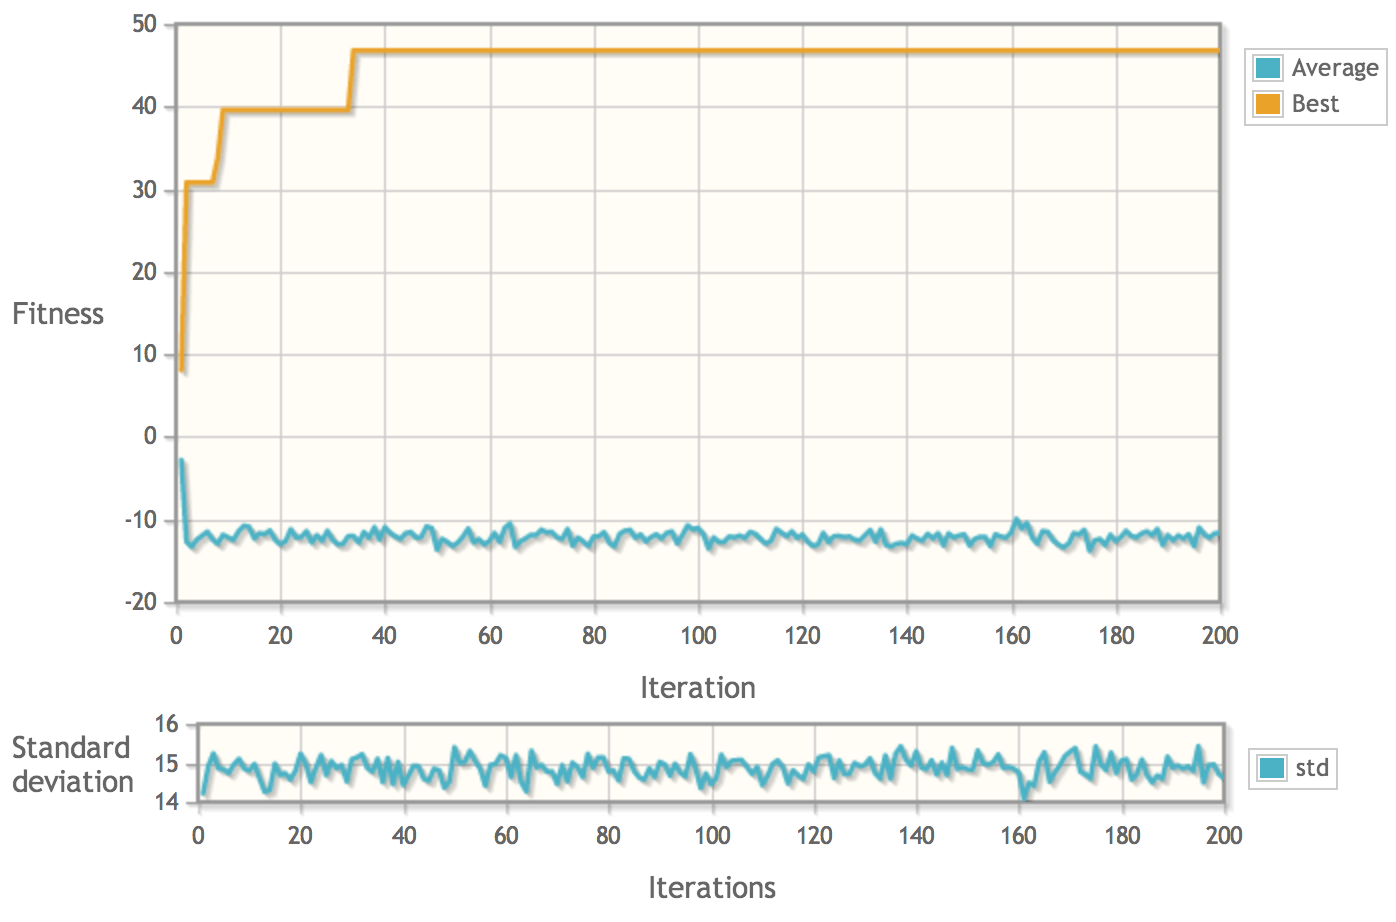
\includegraphics[width=0.6\textwidth]{img/tracker_mainrun}
    \caption{Fitness plot of a successful run with the EA parameterers and the fitness function given above}
\end{figure}

\subsection{Parameteres to catch all objects}
To catch all types of objects it was just to modify the fitness function to penalize misses and give credits for negatives, in change from the other fitness function. The catch all fitness function we used was:

\begin{center}
$f(h,p,m,n) = h + n + p - m$
\end{center}


\begin{figure}[h]
  \centering
    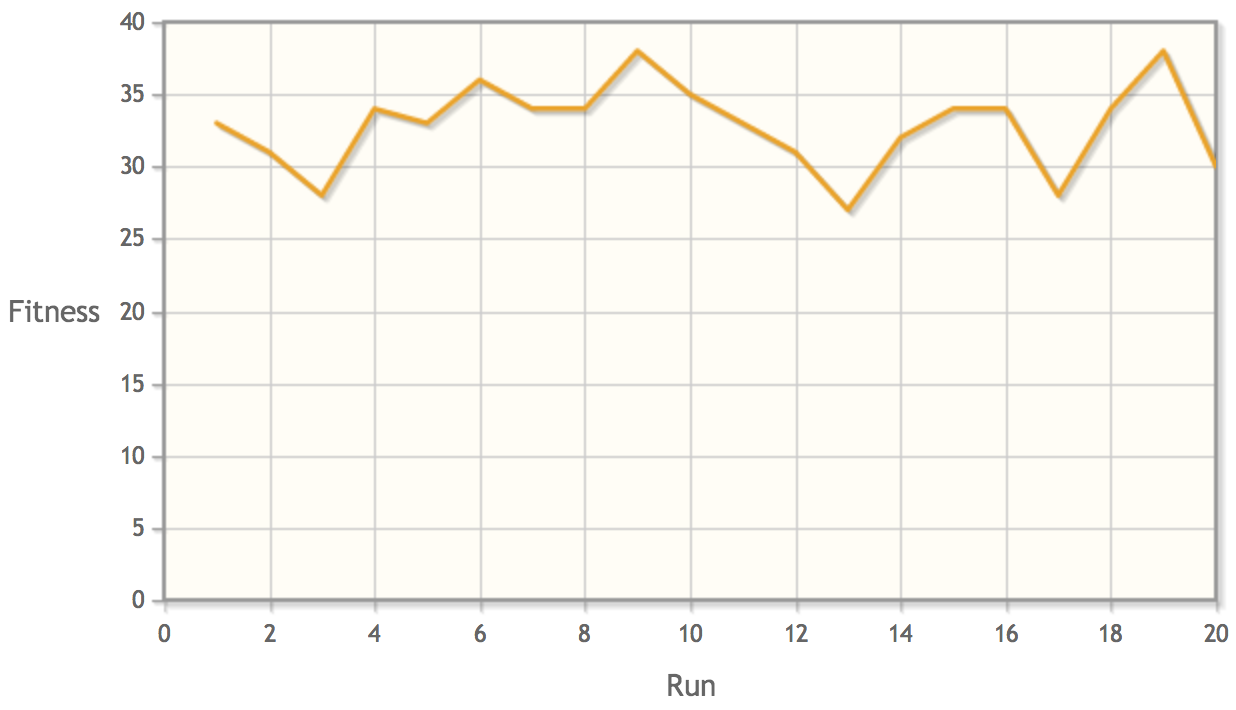
\includegraphics[width=0.8\textwidth]{img/catch_all}
    \caption{20 runs with the catch all fitness function. All runs is well above 25, and the most is over 30. A miss of one object will penalize off by 2 from the best score, 40.}
\end{figure}


\subsection{Significant modifications}
\subsubsection{Tracker scenario}
We changed the world width to be double the original size (60 units). The Tracker agent did the same job as in the normal case. This change is a fairly small change as long as the agent have the ability to move fast inside the evolved genotype. 

\subsubsection{CTRNN variables}
We changed the conversion of the weights to have the range of $w_{i,j} \in [-100, 100]$. This resulted in a very restless behaviour in the agent. The agent moved very often 2+ moves in a step. The result of this change had a bad influence on the catching of the small objects falling sideways. We think this can possible happen because the weights passing through the network will be high and the output sensors will have a relatively high number to normalize to the moving range (-4 up to 4). The final input to the output nodes will have a lot of noise to deal with. 


\subsection{Weight analysis}
tekst tekst tekst


Fitness = 43.0
\begin{figure}[h]
  \centering
    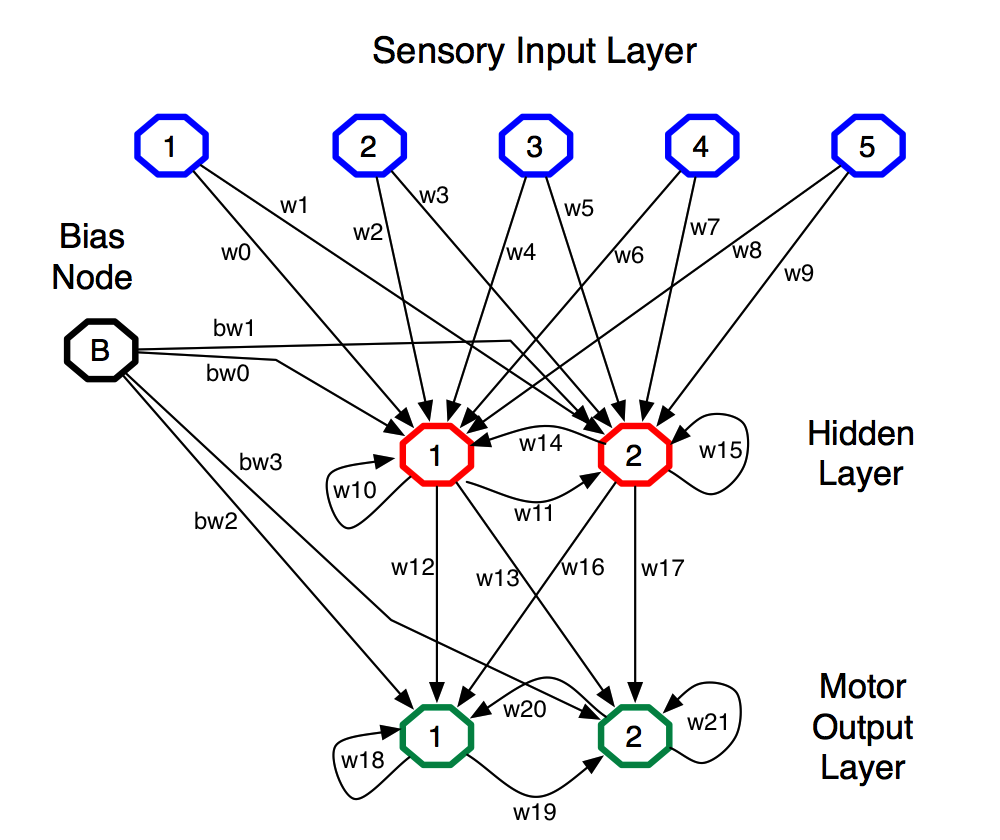
\includegraphics[width=1.0\textwidth]{img/CTRNN}
    \caption{The CTRNN network used in the Tracker agent}
\end{figure}

\begin{tabular}{c | c | c | c | c | c | c | c | c | c | c | c | c }

w0  & w1  & w2  & w3  & w4  & w5  & w6  & w7  & w8  & w9  & w10 & w11 & w12 \\
\hline
2.22 & -1.83 & -0.49 & -0.8 & 0.88 & -3.59 & -4.6 & 0.10 & -1.90 & 2.02 & 2.06 & 0.019 & -0.33 \\ \\

w13 & w14 & w15 & w16 & w17 & w18 & w19 & w20 & w21 & bw0 & bw1 & bw2 & bw3 \\
\hline
4.02 & 5.0 & 1.31 & 2.8 & 4.96 & -3.59 & -4.84 & 4.84 & -0.61 & -8.7 & -6.24 & -7.69 & -0.55 \\

\end{tabular}



\begin{tabular}{l | l}
	input & ouput \\ \hline
	(0, 0, 0, 0, 0) & 2 \\
    (0, 0, 0, 0, 1) & 1  \\
    (0, 0, 1, 0, 0) & -2 \\
    (0, 1, 0, 0, 0) & 2 \\
    (0, 0, 1, 1, 1) & 1  \\
    (1. 0, 0, 0, 0) & -2 \\
    (1, 1, 1, 0 ,0) & -1 \\
    (0, 0, 1, 1, 1) & 1  \\
\end{tabular}


When no inputs are given we see that the trackers motor output is stabilizing on a constant value. Whenever an input is triggered the value is immediatly propagated through the network and changes the motoroutput. We can tell that the EA has evolved a tracker that preferred to just hit an object on the leftmost and rightmost blocks on the tracker. We can tell this by the weights w0 and w9, which have higher values than the others. When no inputs are given the biasnode is the one who decides where the tracker should go.



